% Note to reader: lines beginning with the '%' character are
% 'comments' to you, the human reader of this code, and are 
% ignored by the LaTeX compiler.

%%%%%%%%%%%%%%%%%%%%%%%%%%%%%%%%%%%%%%%%%%%%%%%%%%%%%%%%%%%%%%%%%%
% = Sample template for MIT Junior Lab Student Written Summaries =
% Available from 
%    http://web.mit.edu/8.13/www/Samplepaper/sample-paper.tex
%
% Last Updated July 23, 2014
%
% Adapted from the American Physical Societies REVTeK-4.1 Pages
%    at http://publish.aps.org
%
% ADVICE TO STUDENTS: Each time you write a paper, start with this
%    template and save under a new filename.  If convenient, don't
%    erase unneeded lines, just comment them out using the 
%    '%' character at the start of the line.  Often, they
%    will be useful containers for information.
%
% Using pdflatex, images must be either PNG, GIF, JPEG or PDF.
%    Turn EPS (encapsulated postscript) images to PDF using the
%    epstopdf utility on UNIX systems.
%%%%%%%%%%%%%%%%%%%%%%%%%%%%%%%%%%%%%%%%%%%%%%%%%%%%%%%%%%%%%%%%%%

%%%%%%%%%%%%%%%%%%%%%%%%%%%%%%%%%%%%%%%%%%%%%%%%%%%%%%%%%%%%%%%%%%
% = TO COMPILE THIS DOCUMENT =
%
% From the command line, it would go like this --- assuming you are
%    in the directory where the filename.tex source file and the 
%    filename.bib bibliography file are located, and that you have 
%    permission to create and write files in that directory:
%      > pdflatex filename
%      > bibtex filename
%      > pdflatex filname
%      > pdflatex filename
%    Yes, you run the command several times. The earlier runs 
%    create auxilliary files which keep track of references,
%    citations, equation and section numberring, etc. The later
%    runs combine the information in these auxilliary files with
%    your source document to create the finished product.
%
% If you are using a GUI LaTeX editor like TeXWorks, then there
%    is probably a menu bar button for pdfLaTeX and another for
%    BibTeX. Hit them in the order indicated above. There is 
%    probably also a 'TeXify' button, or something similarly named,
%    which runs all the above commands in one shot.     
%%%%%%%%%%%%%%%%%%%%%%%%%%%%%%%%%%%%%%%%%%%%%%%%%%%%%%%%%%%%%%%%%%


%%%%%%%%%%%%%%%%%%%%%%%%%%%%%%%%%%%%%%%%%%%%%%%%%%%%%%%%%%%%%%%%%%
%  = PREAMBLE =
% The preamble of a LaTeX document is the set of commands that precede
% the \begin{document} line.  It contains a \documentclass line
% to load the REVTeK-4.1 macro definitions and various \usepackage
% lines to load other macro packages.
%
% ADVICE TO STUDENTS: This preamble contains a suggested set of
%     class options to generate a ``Junior Lab'' look and feel that
%     facilitate quick review and feedback from one's peers, TAs,
%     and section instructors.  Don't make substantial changes 
%     to the style without first consulting your section 
%     instructor.
%%%%%%%%%%%%%%%%%%%%%%%%%%%%%%%%%%%%%%%%%%%%%%%%%%%%%%%%%%%%%%%%%%

%\documentclass[aps,twocolumn,secnumarabic,balancelastpage,amsmath,amssymb,nofootinbib, floatfix]{revtex4}
\documentclass[aps,twocolumn,nobalancelastpage,secnumarabic,amsmath,amssymb,nofootinbib,floatfix]{revtex4-1}

%%%%%%%%%%%%%%%%%%%%%%%%%%%%%%%%%%%%%%%%%%%%%%%%%%%%%%%%%%%%%%%%%%%
% N.B.:  Different computers have different packages installed.  
%        To compile this template in the current Athena 
%        environment, REVTeX 4.1 must be used.  To use the older
%        REVTeX 4, switch which documentclass line above is 
%        commented out above. There are ``bad'' distributions of
%        LaTeX for Windows available on the internet which may 
%        cause users to struggle unjustifiably with REVTeX 4.1.
%
%        If you are unable to compile the template at all, you
%        may need to update your LaTeX packages. (Alternatively, if 
%        your LaTeX distribution includes only the older RevTEX 4,
%        then try changing the documentclass line above. In particular,
%        this approach solves a common compilation problem for users of
%        the TeXWorks editor on Windows, which presents erroneously as a
%        error in the bibliography file.) Don't hesitate to speak 
%        with your section instructor or a TA if you're having 
%        issues getting this template to compile.
%%%%%%%%%%%%%%%%%%%%%%%%%%%%%%%%%%%%%%%%%%%%%%%%%%%%%%%%%%%%%%%%%%%

%%%%%%%%%%%%%%%%%%%%%%%%%%%%%%%%%%%%%%%%%%%%%%%%%%%%%%%%%%%%%%%%%%%
% = Explanation of documentclass options =
%
% aps, prl stand for American Physical Society and Physical 
%     Review Letters respectively.
% twocolumn permits two columns, of course.
% nobalancelastpage doesn't attempt to equalize the lengths of 
%     the two columns on the last page  as might be desired in a 
%     journal where articles follow one another closely.
% amsmath and amssymb are necessary for the subequations 
%     environment among others. These functionalities can
%     also be added use the usepackage function described below,
%     but REVTeX conveniently includes them as documentclass
%     options.
% secnumarabic identifies sections by number to aid electronic 
%     review and commentary.
% nofootinbib forces footnotes to occur on the page where they are
%      first referenced and not in the bibliography.
% floatfix attempts to help LaTeX decide where to place ``floats'',
%      like figures and plots, when it gets stuck and can't decide
%      by it's normal algorithm.
% REVTeX 4.1 is a set of macro packages designed to be used with 
%      LaTeX 2e. REVTeX is well-suited for preparing manuscripts 
%      for submission to APS journals.
%
% = Other documentclasses =
%
% The 'revtex4' and 'revtex4-1' documentclasses are somewhat 
%    specialized for making documents in the style of the APS
%    journals. For a more standard or generic looking LaTeX paper,
%    you could try any of the built-in documentclasses, in 
%    particular 'article' or 'report'. Someday, you may try to use 
%    the 'mitthesis'  documentclass available for download from the 
%    MIT Libraries. The vast majority of source code written for 
%    one documentclass should work just fine in any other, but 
%    occasional quirks arise. For example, some documentclasses 
%    disagree on whether the abstract declaration should come 
%    before or after the \begin{document} declaration.
% 
%%%%%%%%%%%%%%%%%%%%%%%%%%%%%%%%%%%%%%%%%%%%%%%%%%%%%%%%%%%%%%%%%%%

%% Now, include some packages which provide new commands that 
%% extend LaTeX's capabilities. Note that the nearly-essential
%% AMS math packages were added already as documentclass options
%% for REVTeX, but could have been added here using 
%% \usepackage{amsmath}, etc. The pacakges below are commonly 
%% useful, but there are many, many more available to solve a 
%% multitude of typesetting quandries (google your problem), 
%% and you  probably have the necesary packages installed on your
%% system already. Among the examples listed below, this sample
%% document only actually makes use of the 'graphicx', 'bm', 
%% and 'hyperref' pacakges, so the others are commented out for
%% tidyness.


\usepackage{graphicx}      % tools for importing graphics
\usepackage{lipsum}
\usepackage{float}
%\usepackage{lgrind}        % convert program code listings to a form 
                            % includable in a LaTeX document
%\usepackage{xcolor}        % produces boxes or entire pages with 
                            % colored backgrounds
%\usepackage{longtable}     % helps with long table options
%\usepackage{epsf}          % old package handles encapsulated postscript issues
\usepackage{bm}            % special bold-math package. usge: \bm{mathsymbol}
\usepackage{physics}
\usepackage{tensor}
\usepackage{gensymb}
%\usepackage{asymptote}     % For typesetting of mathematical illustrations
%\usepackage{thumbpdf}
\usepackage[colorlinks=true]{hyperref}  % this package should be added after 
                                        % all others.
                                        % usage: \url{http://web.mit.edu/8.13}


%%%%%%%%%%%%%%%%%%%%%%%%%%%%%%%%%%%%%%%%%%%%%%%%%%%%%%%%%%%%%%%%%%%
% And now, begin the document...
%%%%%%%%%%%%%%%%%%%%%%%%%%%%%%%%%%%%%%%%%%%%%%%%%%%%%%%%%%%%%%%%%%%

\begin{document}
\title{Detection of High-Angle Alpha Particle Scattering through Gold Foil}
\author{Henry Shackleton}
\email{hshackle@mit.edu}
\date{\today}
\affiliation{MIT Department of Physics}


\begin{abstract}
  Thomson's "plum pudding" and Rutherford's hard core models of atomic structure differ in the predictions they make with regards to high-angle scattering. By observing the scattering rates of $\alpha$ particles through gold foil and comparing the trends to theoretical predictions, we are able to conclude that Rutherford's model accurately describes the data acquired.
\end{abstract}

\maketitle
\section{Introduction}
In the beginning of the 20th century, physicists had begun to determine the structure of atoms. J.J. Thomson had discovered the presence of electrons - negatively charged particles with a mass much less than the overall mass of the electron - using cathode rays\cite{electron}. Thomson further hypothesized that the full structure of the atom consisted of electrons surrounded by a "soup" of positive charge. This structure predicts small deflections during scattering events, detailed further in Section II. This behavior was tested by Ernest Rutherford, and experimental results were shown to disagree with Thomson's predictions. To reflect newfound results, Rutherford proposed a new model of the atom, the Rutherford model, which consisted of a densely-packed positive charge (now known as a \textit{nucleus}) in the center. This refutal of Thomson's "plum pudding" model in favor of this alternative theory  was a crucial step in the progress towards our modern day understanding of the atom.

In this experiment, we measure the scattering of $\alpha$ particles emitted from an $\tensor*[^{241}]{\text{Am}}{}$ source through gold foil. Through geometric considerations and calibration procedures, we determine the data trends that both the Rutherford and Thomson theories predict for our measurements. Finally, by comparing the two predictions to our experimental data, we conclude that Rutherford scattering is able to successfully describe our data.

\section{Theoretical Background}
Scattering processes are typically described by their \textit{differential cross section}, $\dv{\sigma}{\Omega}$. This expression relates, given a scattering process between two particles, the differential size of a cross section and the differential range of the scattered particle. This function is proportional to the probability of such a scattering event to occur. As such, translation from differential cross section to observed scattering rates depends on other parameters, such as the incoming flux of particles, the density of our scattering material, and so on. However, these factors contribute multiplicative constants to the differential cross section, and we will take them to stay the same throughout our experiment - therefore, our differential cross section will be assumed to be proportional to our counting rate.

In the case of Rutherford's model of the atom, scattering processes are given by Coulomb interactions between the nucleus of incoming atom and the nuclei of the atoms in the scattering material. The electrons, while negatively charged, are too light to produce scattering effects. Furthermore, the atoms in the scattering material are assumed to be fixed, reducing the calculation to our incoming charged particles scattering off stationary charges. The differential cross section is given by
\begin{equation}
  \dv{\sigma}{\Omega} = \left(\frac{Z Z' e^2}{16 \pi \epsilon_0 E}\right)^2 \frac{1}{\sin^4(\theta/2)}
  \label{rutheq}
\end{equation}
where $Z$ and $Z'$ are the atomic numbers of the incoming particle and scattering material, respectively, $e$ is the charge carried by a proton, $E$ is the incoming energy of the particle, and $\theta$ is the angle at which our particle scatters. This equation indicates that, assuming the energy of our incident particles is constant, our scattering rate at an angle $\theta$ will be proportional to $1/\sin^4(\theta/2)$.

Rutherford scattering is derived assuming only \textit{one} scattering event between incident particles and scattering material. This approximation is valid for large angles, where the frequency of atoms scattering off multiple particles is low relative to the frequency of single scatterers. However, this is not the case for small angles, and in this regime, our Rutherford formula breaks down. While this multiple angle scattering can be described in the Rutherford framework \cite{scatter}, the relationship is much more complex. For this reason, we only measure large angle scatterings, where Equation \ref{rutheq} is valid in the Rutherford model.

Thomson's "plum pudding" atomic model, absent of any dense concentration of positively or negatively charged particles, does not predict large angle scattering at as high of a rate as the Rutherford theory. Scattering is produced only from weak Coulomb interactions as particles pass by each other. This leads to a predicted scattering rate
\begin{equation}
  \dv{\sigma}{\Omega} \propto e^{-\theta^2/\theta_m^2}
\end{equation}
Where $\theta_m$, the \textit{mean multiple scattering angle}, controls how quickly scattering dies off at large angles. In the case of gold foil, $\theta_m \approx 1\degree$. 

\section{Experimental Setup}
Our apparatus consists of an $\alpha$ particle howitzer, a gold foil, and a silicon barrier detector, all enclosed in a vacuum, sustained at a pressure between 50 and 100 microns. Inside the $\alpha$ particle howitzer is an $\tensor*[^{241}]{\text{Am}}{}$ source, which emits $\alpha$ particles (a collection of two protons and two neutrons) at discrete energies, the most common of which being 5.486 MeV (86\%) an 5.443 MeV (12.7\%). However, a gold coating installed on the cover of the Am source reduces this energy to 4.84 MeV \cite{sean}.The geometry of the howitzer allows for a directed beam of $\alpha$ particles to be emitted, as shown in Figure \ref{apparatus}. The sustained vacuum prevents energy loss of these particles through the air, as well as reducing the frequency of noise in our experiment.
\begin{figure}[h]
  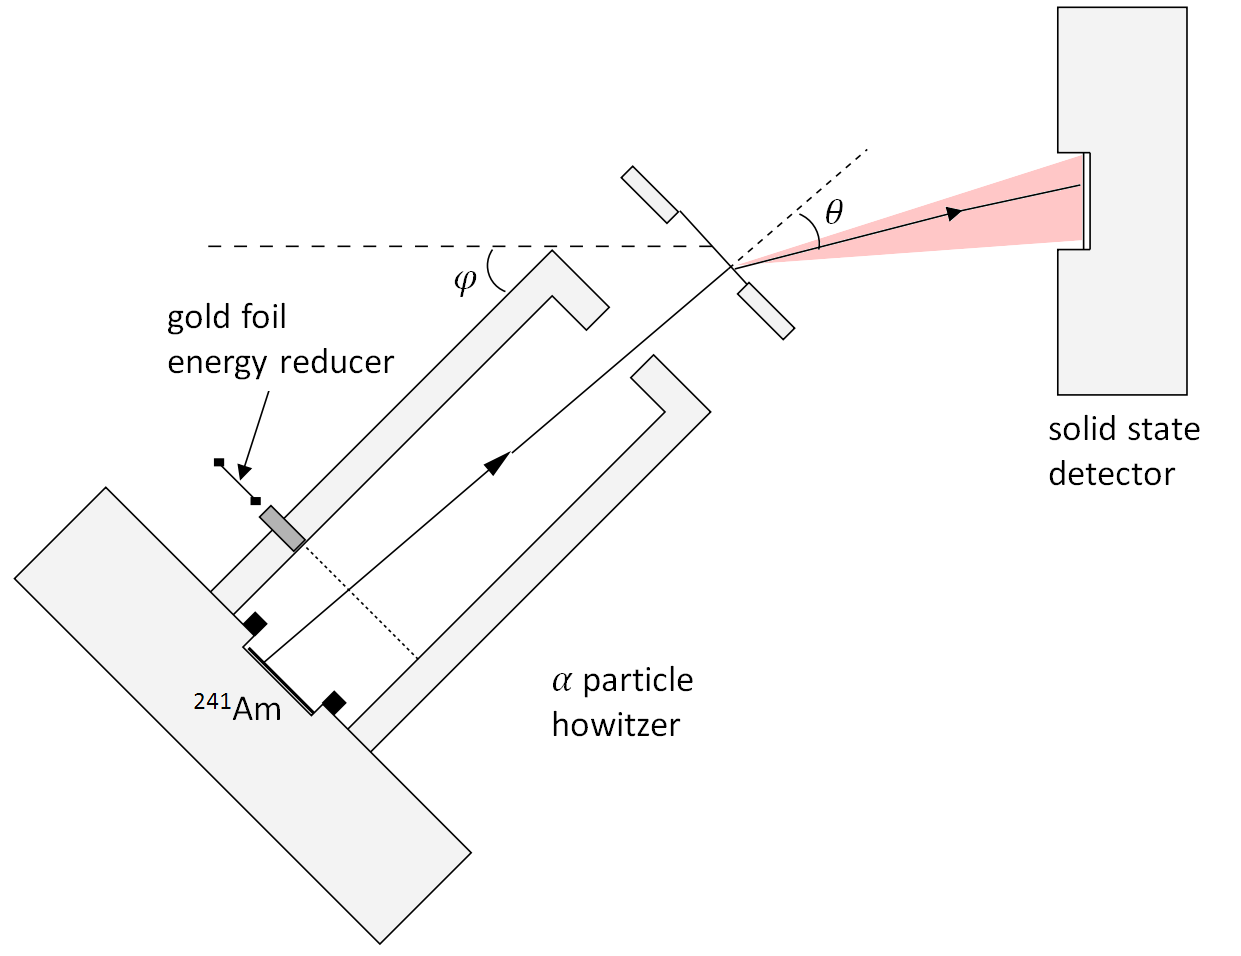
\includegraphics[width=0.5\textwidth]{apparatus-width1.png}
  \caption{An overhead view of our apparatus, detailing the howitzer, gold foil, detector, and the geometric relations between the three \cite{jlab}. The range of angles that can be measured due to the width of our detector is highlighted in red.}
  \label{apparatus}
\end{figure}
This beam of $\alpha$ particles is directed at a gold foil, where the particles are scattered off at some angle $\theta$. These particles can then be detected by our detector, which sends collects the particle's energy and sends it to an MCA to be analyzed. Our howitzer and gold foil is positioned at an angle $\varphi$ away from the detector, measured by a protractor placed inside the apparatus. Because this protractor is read by eye, any angular measurement has an associated uncertainty of $\pm 1\degree$. 

Assuming the detector and beam size were infinitesimally small, the scattering angle of our detected particles would be constrained to $\theta = \varphi$. However, our detector has a width of approximately 1.3 cm, which allows our detector to measure particles scattered at angles around $\varphi$. This geometric relation is shown in Figure \ref{apparatus}. Additionally, our beam width of approximately 0.63 cm allows for further scattering angles outside of $\varphi$ to be measured.

These features of our apparatus can be captures by the \textit{angular response function}, $g(\varphi, \theta)$. This function describes, given that our howitzer is positioned at an angle $\varphi$, the probability of a detection having been from a particle scattered at an angle $\theta$. Given our theoretical scenario of point detectors and sources, we would simply have an angular response function of
\begin{equation}
  g(\varphi, \theta) = \delta(\theta - \varphi)
\end{equation}
As a first approximation, we expect the probability of detection to fall off linearly away from $\varphi$, so we approximate the form of $g(\varphi, \theta)$ to be a triangle. To determine the width of this triangle, we remove the gold foil from our apparatus, and measure how changes in $\varphi$ affect our count rate. This distribution is equivalent to $g(0, \theta)$. Our measured data, along with a triangle fit, is displayed in Figure \ref{profile}. This graph gives us the general form of $g(\varphi, \theta)$ - replacing the $\theta=0\degree$ point with the howitzer angle $\phi$ gives the distribution around $\varphi$ of scattering angles detected. Figure \ref{profile} also indicates that the protractor in our apparatus is slightly off-center - we would expect the maximum counting rate to be when the howitzer is pointed straight at the detector, or at $\varphi = 0$\degree, but instead, this occurs at around $\varphi = -2\degree$.

As the reduced $\chi^2$ of this fit is poor, and we can see by eye that the data follows a rough Gaussian trend, we fit to a Gaussian distribution as well as a triangle. This gives a reduced $\chi^2$ of $0.246$, with  $\sigma = 2.73 \pm 19$ and $\mu = -1.819 \pm 0.29$. This low reduced $\chi^2$ may be a sign of overfitting, as we have no reason a priori to assume a Gaussian fit. Nevertheless, we include it to examine the effects it has on our final answer.
\begin{figure}[h]
  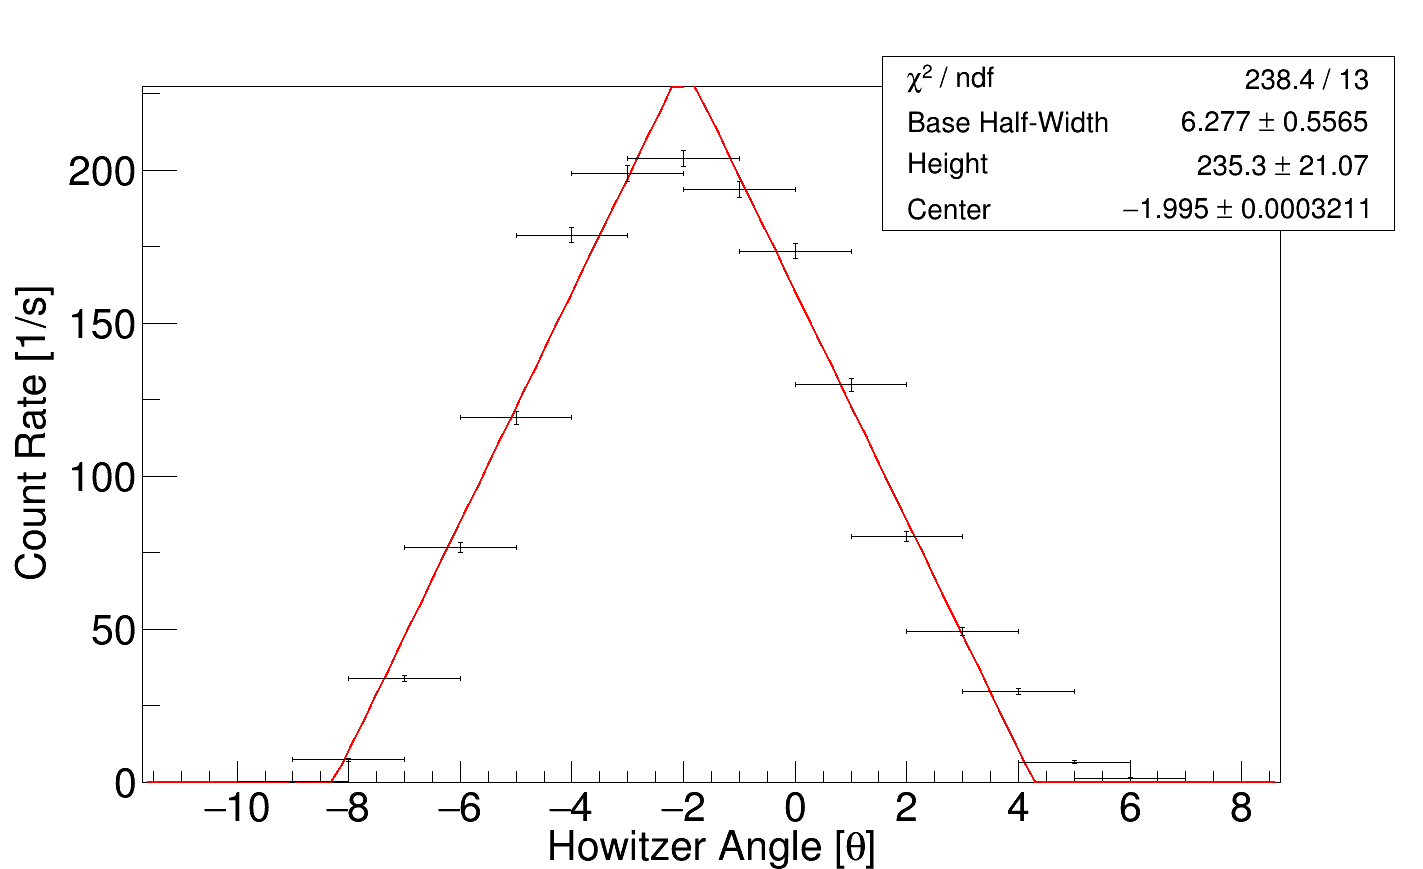
\includegraphics[width=0.5\textwidth]{c1.png}
  \caption{The count rate of our particles, with each data point acquired over the course of 300 seconds. A triangle function is fit to our distribution. The goodness of fit is not perfect, indicating that our modeling of our angular response function as a triangle is only an approximation.}
  \label{profile}
\end{figure}

To calculate how this angular response function affects our observed counting rates, we convolve $g(\varphi, \theta)$ with the predicted scattering rates for both Rutherford and Thomson theories, as shown in Equation \ref{convolveeq} (note that, as we are solely concerned with the angular dependence, the various constants have been replaced by one constant, $C_0$). This convolution can be thought of as taking the probability of a particle being scattered at an angle $\theta$, multiplying it by the probability of the detector positioned at an angle $\varphi$ to detect this scattering, and integrating over all $\theta$. The end result is two counting rates, $C_r(\varphi)$ and $C_t(\varphi)$, which are the predicted counting rates with our howitzer at an angle $\varphi$ predicted by the Rutherford and Thomson models, respectively.

\begin{equation}
  \begin{aligned}
    C_r(\varphi) &= C_{r,0}\int\limits_0^\pi g(\varphi, \theta) \sin^{-4}(\theta/2) \dd{\theta}
    \\
    C_t(\varphi) &= C_{t,0} \int\limits_0^\pi g(\varphi, \theta) e^{-\frac{\theta^2}{\theta_m^2}}  \dd{\theta}
    \label{convolveeq}
  \end{aligned}
   \end{equation}


   \section{Data Analysis}
   Over the course of our experiment, we took scattering measurements through gold foil at howitzer angles between $10\degree$ and $60\degree$. Our MCA readout for all measurements followed trends similar to the distribution shown in Figure \ref{mca}. The distribution of our energy loss can be fitted to Landau distribution, with is be done for all our runs with a reduced $\chi^2$ ranging from 0.57 to 0.88. As a Landau distribution is the predicted energy loss distribution for particles travelling through material\cite{landau}, this confirms that all or nearly all data collected is from scattering.

   Noise for our experiement is measured by pointing the howitzer well away from the detector and collecting data. This data shows minimal noise in our experiment, most of it with energies below our area of interest. For energies within this range, we measure an average counting rate of noise as $0.0002 \pm 0.00018$ counts/second. This rate is not comparable to any of the counting rates we observe, and as such, can be disregarded. This further confirms that nearly all counts acquired were from scattering events.
   \begin{figure}[h]
     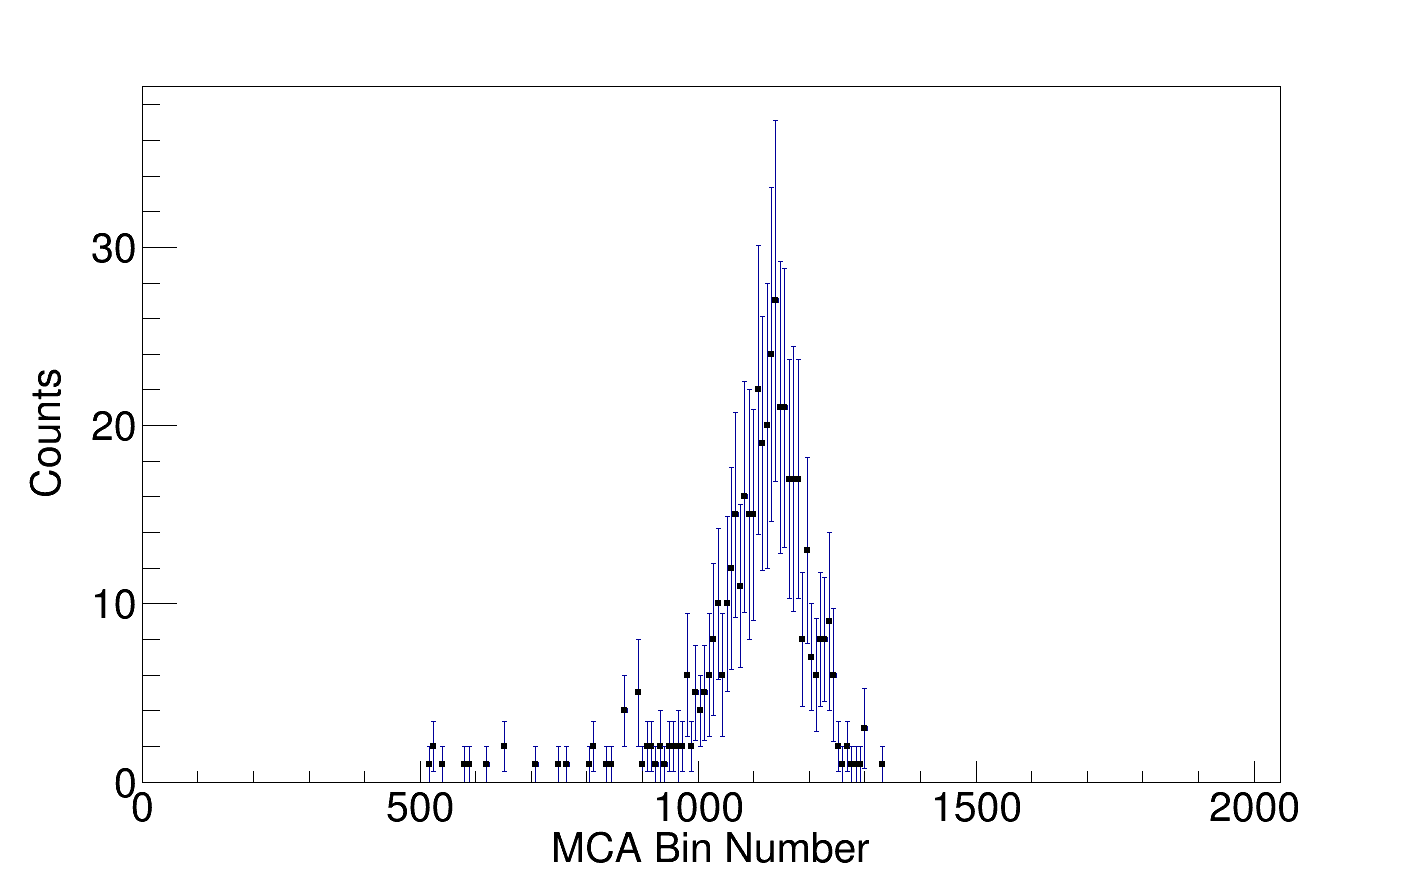
\includegraphics[width=0.5\textwidth]{mca_readout.png}
     \caption{The MCA readout for our scattering measurement at $\varphi = 20\degree$. The MCA bin number corresponds linearly to the energy of the measured events.}
     \label{mca}
   \end{figure}

   Further analysis of this Landau-distributed energy loss allows us to calculate the thickness of our gold foil. As the energy of $\alpha$ particles passing through a vacuum is known to be 4.84 MeV, taking $\alpha$ particle measurements with the gold foil removed and analyzing the distribution allows us to determine which MCA bin number corresponds to this 4.84 MeV  energy. This, combined with the assumption that the zero MCA bin number corresponds to zero energy, allows for a linear fit and a complete correspondance between MCA bin number and detected energy, with some uncertainty due to the width of the peak observed in the vacuum measurement. 

   With this calibration, we are able to determine the mean energy of our particles after passing through gold foil. This allows us to calculate the energy loss through gold foil as $0.80 \pm 0.04$ MeV. We acquire data on the stopping power of gold - the rate of energy loss of an $\alpha$ particle through gold - from the NIST database, displayed in \ref{stop}. Dividing our energy loss by this rate, we are able to determine the distance through the gold that our $\alpha$ particles travel, and hence calculate the thickness of our gold foil as $1.68 \pm 0.08 \mu$m. This falls within $3\sigma$ of the reported thickness, $1.3 \pm 0.1 \mu$m.

   \begin{figure}[h]
     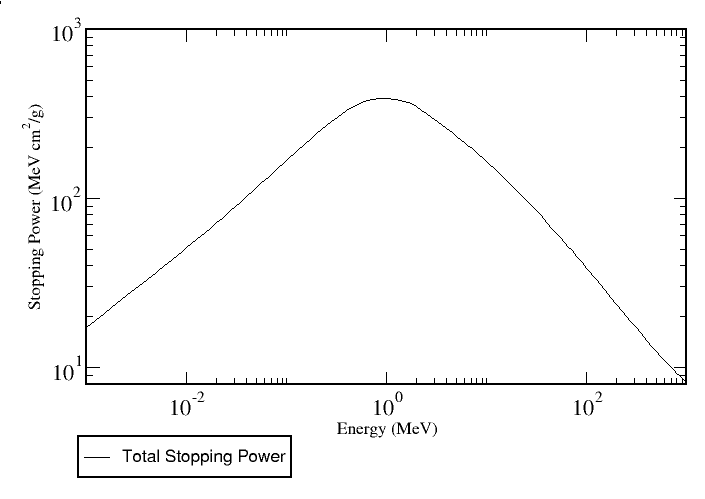
\includegraphics[width=0.5\textwidth]{nist.png}
     \caption{The stopping power for $\alpha$ particles passing though gold, as a function of the energy of the $\alpha$ partices. To calculate the average stopping power, we determine both the stopping power at the incident energy of the $\alpha$ particle and the stopping power at the final energy of the $\alpha$ particle, and take the average.}
     \label{stop}
   \end{figure}

Taking the number of counts detected at each angle and their associated Poissonian uncertainty, we divide by the time of acquisition to determine the counting rate at a given howitzer angle. These scattering rates are plotted as a function of their howizter angle position, and then fitted to the Rutherford and Thomson models convolved with a triangle. The results of these fits is displayed in Figure \ref{final-plot}.

\begin{figure}[h]
  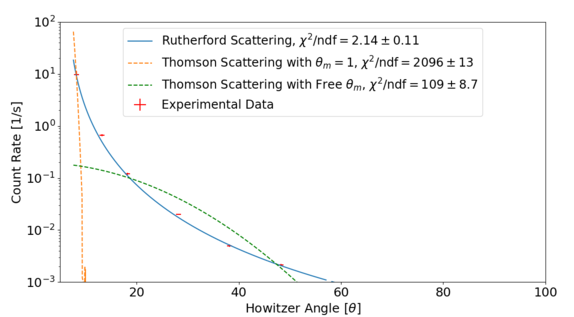
\includegraphics[width=0.5\textwidth]{plot-error.png}
  \label{final-plot}
  \caption{Experimentally-measured scattering rates plotted against their howitzer angle are fitted to the rates predicted by both Rutherford and Thomson. Thomson's model, even with $\theta_m$ as a free parameter, is unable to predict the slow falloff of scattering rates at large angles.}
\end{figure}
As clearly shwon by Figure \ref{final-plot}, Thomson's plum pudding model is unable to predict these high-angle scattering rates. For a more complete analysis, we consider both the Thomson model with the mean multiple scattering angle fixed at the usual $\theta_m = 1$ as well as with $\theta_m$ as a free parameter. However, it is clear that the exponential falloff predicted by Thomson's model leads to a fundamentally different shape in the predicted counting rate than Rutherford's $1/\sin^4(\theta/2)$ dependence.

\begin{figure}[h]
  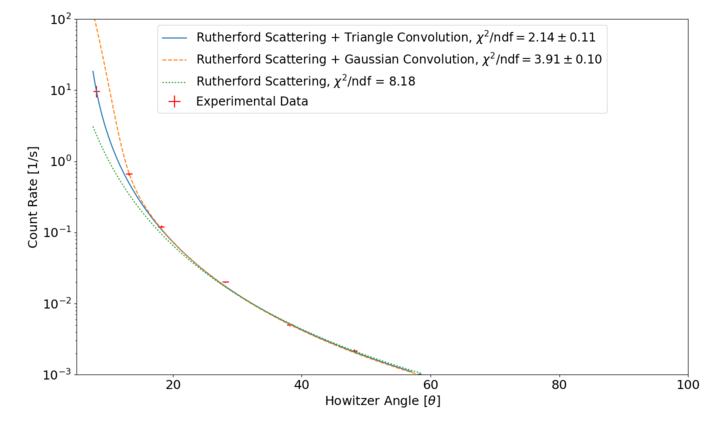
\includegraphics[width=0.5\textwidth]{gaus.png}
  \label{convdata}
  \caption{A visual comparison of our data fitted to the raw Rutherford formula, a triangle convolution, and a Gaussian convolution. While all three capture the overall trends of our data, the triangle convoluted Rutherford formula more accurately fits our data.}
\end{figure}


The geometric considerations and calibration measurements in Section III lead to a triangle function to be convolved with our predicted scattering rates. Hoewver, the parameters on this triangle come with some uncertainty. The effect of this uncertainty on our goodness of fit can be approximated by varying the parameters and determining our $\chi^2$'s dependence on them. The variation in these reduced $\chi^2$'s are reported in Figure \ref{final-plot}.


Further analysis of the effects of our convolution is necessary to confirm that our triangle approximation is valid. For this, we fit our data to both an unconvoluted Rutherford scattering rate, and a Rutherford scattering rate convoluted with our Gaussian distribution from Section III. The results of this are displayed in Figure \ref{convdata}. While both are not as poor of fits as the Thomson model, as all three capture the approximate trends of our data, the triangle convolution does fit better than both, suggesting that our triangle approximation of the apparatus's angular response function was valid. In future experiments, one would expect that by refining Figure \ref{profile} with further data, one would gain an even more accurate understanding of the apparatus's angular response function.

\section{Conclusion}
By measuring the scattering rates of $\alpha$ particles through gold foil, we are able to determine that Rutherford's scattering formula describes our data more accurately than Thomson's predictions from his plum pudding model. As such, we can conclude tha the atomic structure is more closely described by Rutherford's model than Thomson's. Through geometric considerations and calibration techniques, we are able to account for a systematic effects of our apparatus through a convolution, which is verified to improve the goodness of fit of the Rutherford prediction.

\section{Acknowledgements}
I would like to thank my lab partner, Adin Hrnjic, for his extensive help and advice throughout this project. Discussions with him on error sources, analysis techniques, and scattering theory were invaluable. I would also like to thank the 8.13 staff for their assistance, both technical and with regards to analysis, throughout this experiment.
\bibliography{rutherford-paper}
\end{document}
